\documentclass[../stats.tex]{subfiles}
\graphicspath{{\subfix{../figures/}}}
\begin{document}
\chapter{Inference for Categorical Data: Proportions}
\section{Constructing a One Proportion z-Interval}
Definition: A confidence interval for a population parameter is an interval of plausible values for that unknown parameter.

It is constructed in such a way so that, with a chosen degree of confidence, the value of the parameter will be captured inside the interval.

The chosen degree of confidence is called the confidence level. The confidence level gives information about how much ``confidence'' we have in the method used to construct the interval.

Interpreting a Confidence Level:
\begin{itemize}
    \item If we were to select many random samples {$n$ in context} and construct a \blank \% confidence interval using each sample, about \blank \% of the intervals would capture the {parameter in context}.
\end{itemize}

To create an interval of plausible values for a parameter, we need two components:
\begin{itemize}
    \item A point estimate is a single value used to estimate the population parameter such as a sample proportion.
    \item A margin of error represents the maximum expected difference between the two population parameter and the sample estimate.
\end{itemize}
\begin{center}
    point estimate $\pm$ marging of error 
\end{center}
\begin{center}
    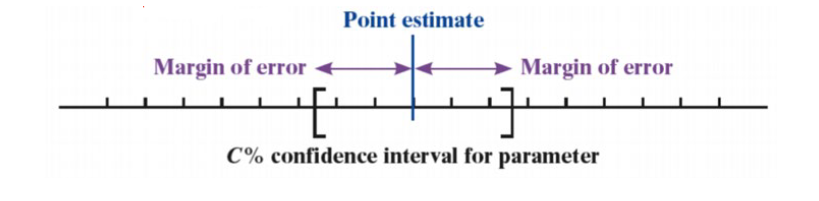
\includegraphics[width=0.8\textwidth]{6.1.1.PNG}
\end{center}

Constructing a Confidence Interval 
\begin{center}
    \begin{tabular}{c|c}
        P & Define the Parameter\\\hline 
        A & Check the Assumptions and Conditions\\\hline
        N & Name the Inference Method \\\hline
        I & Calculate the Interval \\\hline 
        C & Write your Conclusion in Context 
    \end{tabular}
\end{center}

\begin{itemize}
    \item Define the parameter 
    
    $p$ = true proportion of {parameter in context}

    \item Check the Assumptions and Conditions 
    \begin{itemize}
        \item Random Condition: The sample should be a random sample of the population.
        \item 10\% Condition: The sample size, $n$, must be no larger than 10\% of the population.
        \item Success/Fail Condition: The sample has to be large enough so that there are at least 10 success and 10 failures. 
        \begin{center}
            $n\hat{p}\geq 10 \qquad n(1-\hat{p})\geq 10$
        \end{center}
        \item The value of the true population proportion ($p$) is unknown so we use the sample proportion $(\hat{p})$
    \end{itemize}
    \item Name the Inference Method:
    \begin{itemize}
        \item Method: One Proportion z-Interval
    \end{itemize}
    \item Calculate the Interval 
    \begin{center}
        point estimate $\pm$ marging of error 

        $\hat{p}\pm z^*\sqrt{\frac{\hat{p}(1-\hat{p})}{n}}$
    \end{center}
    Recall: The value of the true population proportion $(p)$ is unknown so we use the sample proportion $(\hat{p})$.
\end{itemize}
How do we calculate the Critical Value ($z^*$)
\begin{center}
    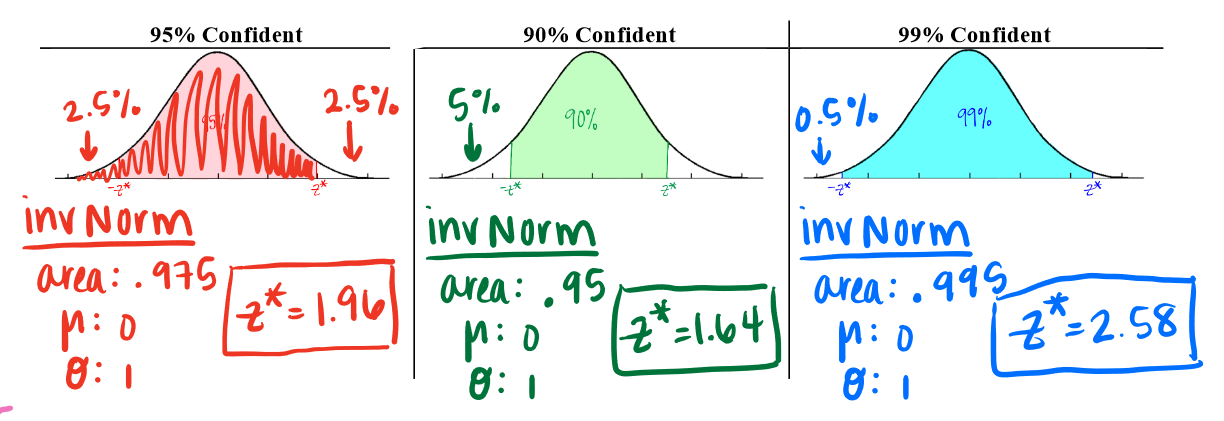
\includegraphics[width=0.8\textwidth]{6.1.2.PNG}
\end{center}
\begin{itemize}
    \item Write your Conclusion in Context 
    \begin{itemize}
        \item We are \blank \% confident that the interval from \blank to \blank captures the true proportion of {parameter in context}.
    \end{itemize}
\end{itemize}

\begin{example}
    A New York Times poll asked a random sample of 400 US adults the question, ``Do you favor an amendment to the Constitution that would permit organized prayer in public schools?'' Based on this poll, the 95\% confidence interval for the population proportion who favor such an amendment is $(0.63,0.69)$.

    (a) Interpret the confidence interval in context.

    We are 95\% confident that the interval from 0.63 to 0.69 captures the true proportion of US adults who favor the amendment.

    (b) Interpet the confidence level in context.

    If were to select many random samples of 400 US adults and construct a 95\% confidence interval using each sample, about 95\% of them would capture the true proportion of US adults who favor the amendment.

    (c) What is the point estimate that was used to capture the interval? What is the margin of error?

    The point estimate is $\hat{p} \pm$ margin of error.

    The marging of error is $\frac{0.69-0.63}{2}=0.03$.

    The point estimate point estimate is therefore $\hat{p}=0.63+0.03=0.66$.

    (d) Based on this poll, a reporter claims that more than two-thirds of US adults favor such an amendment. Use the confidence interval to evaluate this claim.

    Their claim is incorrect, our confidence interval states that the true proportion could also be below 0.67.
\end{example}

\pagebreak
\begin{example}
    In a random sample of 250 Texas high school students, it was found that 210 of them later graduated. Calculate and interpret a 95\% confidence interval to estimate the proportion of all Texas high school students who graduate.

    $p$ = true proportion of Texas HS students who graduate 

    Random sample of 250 TX HS students: $\hat{p}=\frac{210}{250}=0.84$

    Independence: $n=250\leq 0.10$(all TX HS Students). $\sigma_{\hat{p}}=\sqrt{\frac{0.84(1-0.84)}{250}}=0.0232$

    Normal: $210\geq 10$, $250-210=40\geq 10$, sampling dist. is approx. normal.

    One proportion z-interval.

    $\hat{p}\pm z^*$(std error) = $.84\pm 1.96(0.0232)$. 

    The interval is $(0.7945, 0.8855)$. 

    We are 95\% confident the interval from 0.7945 to 0.8855 captures the true proportion of texas high school students who graduate.
\end{example}

Using your calculator you can do the following.

STAT-Tests-A: 1-PropZInt
\begin{itemize}
    \item $x$: number of successes 
    \item $n$: sample size 
    \item C-Level: Confidence Level 
\end{itemize}

Important: Your number of successes must be whole number otherwise your calculator will give you an error.

\section{Constructing a One Proportion z-Test}
A significance test is another inference method that assesses evidence provided by data about a claim. Significance tests tell us if sample data gives us convincing evidence against a null hypothesis.
\begin{itemize}
    \item A null hypothesis ($H_0$) is the claim being assessed in a significance test. Usually, the null hypothesis is a statement of ``no change from the expected value''.
    \item An alternative hypothesis ($H_A$) proposes what we should conclude if we find the null hypothesis to be unlikely.
\end{itemize}

Hypotheses always refer to the population, not the sample. We use $p$ and not $\hat{p}$.

A p-value is the probability of getting results as extreme or more extreme in the direction of the null hypothesis by random chance alone assuming the claim of the null hypothesis is true.
\begin{itemize}
    \item Small p-values give convincing evidence against the null hypothesis since the result we got is unlikely to occur.
    \item Large p-values fail to give convincing evidence against the null hypothesis since the result we got is likely to occur.
\end{itemize}
Interpreting a P-value.
\begin{itemize}
    \item Assuming that the true proportion of {parameter in context} is {null hypothesis}, there is a {p-value} probability of getting a sample proportion of {alternative hypothesis} just by chance in a random sample of {n w/ units}.
\end{itemize}
\pagebreak
\begin{example}
    Jason claims he makes 85\% of his free throws. Thatcher believes that he makes less than 85\% and just wants to test Jason's claim. Jason shoots 100 free throws and makes 82 of them. A significance test is performed and a p-value of 0.2004 is obtained. Interpet the -value in context.

    Assuming that the true proportion of free throws Jason makes is 85\%, there is a 20.04\% probability of getting a sample proportion of 82 free throws or less just by chance in a random sample of 100 free throws.
\end{example}

The significance level ($\alpha$) is a fixed value that we will regard as the decisive value that determines if the p-value is small or large.
\begin{itemize}
    \item Typically we choose $\alpha=0.05$ which says we need data so strong that it would happen by chance less than 5\% of the time.
\end{itemize}

Constructing a Significance Test:
\begin{itemize}
    \item P: Define the Parameter 
    \item H: State the Hypotheses
    \item A: Check the Assumptions and Conditions 
    \item N: Name the Inference Method 
    \item T: Calculate the Test Statistics
    \item O: Obtain the P-Value 
    \item M: Make a Decision 
    \item S: State the Conclusion in Context 
\end{itemize}

Define the parameter:

$p$ = true proportion of {parameter in context}

State the Hypotheses: 
\begin{itemize}
    \item Null Hypothesis: $H_0: p=p_0$
    \item Alternative Hypothesis:
    \begin{itemize}
        \item $H_A: p<p_0$
        \item $H_A: p>p_0$
        \item $H_A: p\neq p_0$
    \end{itemize}
    If you are not given a claimed proportion, we use a conservative estimate which is 0.50.
\end{itemize}

Check the Assumptions and Conditions 
\begin{itemize}
    \item Random Condition: The sample should be a random sample of the population.
    \item 10\% Condition: The sample size $n$, must be no larger than 10\% of the population.
    \item Success/Fail Condition: The sample size has to be large enough so that there are at least 10 success and 10 failures.
    \begin{center}
        $np_0 \geq 10 \qquad n(1-p_0)\geq 10$
    \end{center}
\end{itemize}

Name the Inference Method: 

Method: One Proportion z-Test 

Calculate the Test Statistic

On the formula chart:
\begin{center}
    test statistic = $\frac{\text{statistics-parameter}}{\text{standard deviation of statistic}}$
\end{center}

One Proportion z-Test
\[ z = \frac{\hat{p}-p_0}{\sqrt{\frac{p_0(1-p_0)}{n}}} \]
Where $\hat{p}$ is sample proportion, $p_0$ is the null proportion, and $n$ is sample size.

Obtain the P-Value 
\begin{center}
    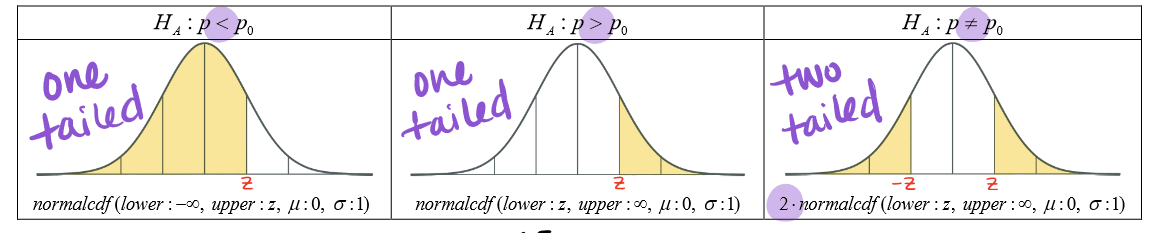
\includegraphics[width=0.8\textwidth]{6.2.1.PNG}
\end{center}

Make a Decision 
\begin{itemize}
    \item If the p-value is less than $\alpha$, we reject the null hypothesis.
    \item If the p-value is greater than $\alpha$, we fail to reject the null hypothesis.
\end{itemize}

Write your Conclusion in Context 

Since our p-value of \blank is (less/greater) than $\alpha = \blank$, we (reject/fail to reject) the null hypothesis. There (is/is not) convincing evidence that {alternative hypothesis}.

\begin{example}
    According to the U.S. Census Bureau, the proportion of students in high school who have a part-time job is 0.25. An administrator at a local high school suspects that the proportion of students at her school 
    who have a part-time job is less than the national figure. The administrator selects a random sample of 200 students from the school and finds that 39 of them have a part-time job. Is there convincing evidence that the proportion of students at the administrator's school who have a part-time job is less than the national figure?

    p = true proportion of students at admin's school with a part time job.

    $H_0: p=0.25$, $H_A: p<0.25$

    \begin{itemize}
        \item Random: Random sample of 200 students at admin's school 
        \item Independence: $n=200\leq 0.10$(all students at admin's school)
        \item Normal: $200(0.25)=50\geq 10$, $200(0.75)=150\geq 10$, sampling dist. is approx. normal.
    \end{itemize}

    One Proportion z-Test 

    $z=\frac{\hat{p}-p_0}{\sqrt{\frac{p_0(1-p_0)}{n}}}=-1.7963$. 

    $P(z<-1.7963)=0.0362$.

    Since the p-value of 0.0362 is less than $\alpha=0.05$, we reject the null. There is convincing evidence that the proportion of HS students with part time jobs is less than the national claim at admin's school.
\end{example}

\pagebreak
\begin{example}
    According to the Centers for Disease Control and Prevention, 68\% of high school students have never smoked a cigarette. Serene wonders if this national figure holds true at her high school. Serene takes an SRS of 150 students from her school.
    She gets responses for all 150 students and 62\% say that they have never smoked a cigarette. Is there convincing evidence that the CDC's claim does not hold true at Serene's school?

    p = true prop. of students at Serene's high school who never smoked a cigarette

    $H_0: p=0.68$, $H_A: p\neq 0.68$

    \begin{itemize}
        \item Random: SRS of 150 students at Serene's school
        \item Independence: $n=150\leq 0.10$(all high school students at Serene's school)
        \item Normal: $150(0.68)=102\geq 10$, $150(1-0.68)=48\geq 10$. Sampling dist. is approx. normal.
    \end{itemize}

    One proportion z-Test 

    $z=-1.5753$, $P(z<-1.5753)=0.0576$.

    Multiply this by two, since the alternative is two tailed, so $p=0.1152$.

    Since the p-value of 0.1152 is greater than $\alpha=0.05$, we fail to reject the null. There is not convincing evidence that the proportion of students at Serene's high school who never smoked a cigarette is different than the CDC's claim.
\end{example}

Calculator Steps:

STAT-Tests-5:1-PropZTest:
\begin{itemize}
    \item $p_0$: null proportion 
    \item $x$: number of successes
    \item $n$: sample size 
    \item prop: alternative hypothesis
\end{itemize}
Important: Your number of successes must be a whole number otherwise your calculator will give you an error.

\pagebreak
\section{Relating Confidence Intervals and Significance Tests}
\begin{example}
    A recent study suggested that 77\% of teenagers have texted while driving. A random sample of 50 teenage drivers at the school was taken and 33 admitted to texting while driving. Assume all conditions have been met. Use your calculator answer the following questions.

    (a) Construct a 99\% confidence interval to estimate the true parameter of teens who text while driving.

    p = true prop. of teens who have texted while driving at this school.

    one proportion z-interval: $(0.4874, 0.8326)$, $\hat{p}=0.66, n=50$.

    We are 99\% confident the interval from 0.4874 to 0.8326 captures the true prop. of teens who have texted while driving at this school.

    (b) Conduct a significance test to determine if the proportion of teens who text while driving is different from 77\%. Use a 1\% significance level.

    $H_0: p=0.77$, $H_A: p\neq 0.77$

    one proportion z-test.

    $z=-1.8483, \hat{p}=0.66, p=0.0646, n=50$.

    Since the p-value of 0.0646 is greater than $\alpha = 0.01$, we fail to reject the null. There is not convincing evidence that the true prop. of teens who text and drive is different than 77\%.

    (c) What type of results did you get for the confidence interval and significance test?

    \begin{itemize}
        \item Confidence interval: Interval of plausible values for $p$
        \item Significance Test: said 77\% is still a plausible value for $p$.
    \end{itemize}
    Confidence interval contains 0.77 which agrees with failing to reject $H_0: p=0.77$.
\end{example}

\begin{center}
    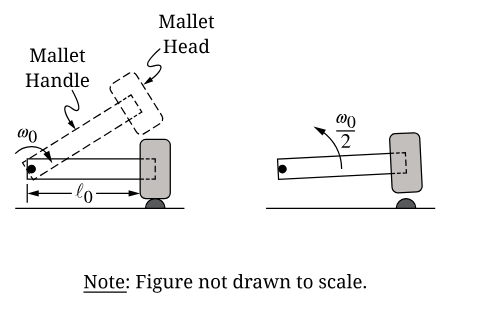
\includegraphics[width=0.8\textwidth]{6.3.1.PNG}
\end{center}
\begin{itemize}
    \item If the confidence interval contains the null hypothesis from a two-sided test, we would fail to reject the null.
    \item If the confidence interval does not contain the null hypothesis from a two-sided test, we would reject the null.
\end{itemize}

\pagebreak
\begin{example}
    Scott's Turf Lawn Builder makes the claim that, when a user plants their grass seeds, 88\% of seeds will germinate. The germination rate of seeds is defined as the proportion of seeds that, when properly planted in the fertilizer and watered, sprout and grow. The company regularly tests this claim, to make sure its product is efficient. 
    They plant 500 grass seeds in their fertilizer and find that 412 of the seeds germinate. Assume that all conditions are met.

    (a) What is the 95\% confidence interval for this observation?

    $(0.7906, 0.8574)$

    (b) Suppose the company conducted a test of $H_0: p=0.88$ against the alternative $H_A: p\neq 0.88$, using $\alpha=0.05$. Use the confidence interval to determine whether this test would reject or failt to reject the null hypothesis. Explain your reasoning.

    Because our 95\% confidence interval does not contain 0.88, we reject the null. There is convincing evidence that the germination rate of seeds is not 0.88.

    (c) Find the p-value for the test. Explain what the p-value measures in the context of the problem.

    $z=-3.8534$, $p=0.001$. Assuming the germination rate is 0.88, there is a 0.0001 prob. of getting $\hat{p}=0.824$ or more extreme just by random chance alone.
\end{example}

\begin{center}
    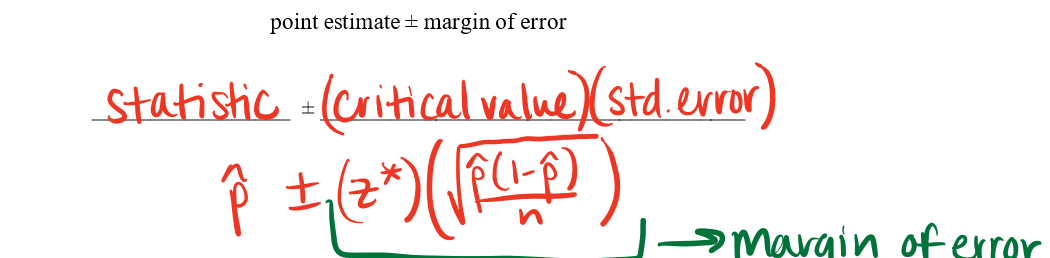
\includegraphics[width=0.8\textwidth]{6.3.2.PNG}
\end{center}

When increasing confidence level 
\begin{itemize}
    \item Critical value increases 
    \item Margin of error increases 
    \item Wider interval 
\end{itemize}

When decreasing confidence level 
\begin{itemize}
    \item Critical value decreases 
    \item Margin of error decreases
    \item Narrower interval 
\end{itemize}

When increasing sample size 
\begin{itemize}
    \item Standard error decreases
    \item Margin of error decreases
    \item Narrower interval 
\end{itemize}

When decreasing sample size 
\begin{itemize}
    \item Standard error increases 
    \item Margin of error increases 
    \item Wider interval 
\end{itemize}

Keep in mind 
\begin{itemize}
    \item The margin of error in a confidence covers only accounts for sampling variability 
    \item The margin of error does not account for bias in the sampling methods 
\end{itemize}

Often time, researchers need to both limit the margin of error to a fixed amount and still maintain a certain confidence level. In such cases, the only thing that can vary is the sample size, since 
the value for $\hat{p}$ is something that is out of our control.

If we know our margin of error and our confidence level, we can solve for $n$ to determine the sample size needed to obtain a certain margin of error size.

However, we don't know $\hat{p}$ until we actually conduct the study.

We can then do one of two things:
\begin{enumerate}
    \item Use an estimated $\hat{p}$ based on previous studies (this would be the wording used in the problem)
    \item Use a ``conservative'' $\hat{p}=0.5$. Using a $\hat{p}$ of 0.5 gives the largest possible margin of error for any given z or n. We will use this option when a value of $\hat{p}$ is not given in the problem.
\end{enumerate}

\begin{example}
    In 2009 a survey of Internet usage found that 79 percent of adults age 18 years and older in the United States use the Internet. A broadband company believes that the percent is greater now than it was in 2009 and will conduct a survey.
    The company plans to construct a 98 percent inverval to estimate the current percent and wants the margin of error to be no more than 2.5 percentage points. Assuming that at least 79 percent of adults use the Internet, how many people must they random sample to achieve this?

    The $z^*$ for a 98\% confidence interval is 2.33.

    We have $0.025\geq 2.33\sqrt{\frac{0.79(1-0.79)}{n}}$, so $n\geq 1441.0472$.

    We need at least 1442 people.
\end{example}

\section{Inference for Comparing Two Population Proportions}
Constructing a two proportion z-interval 

\begin{itemize}
    \item Define the parameter 
    \begin{itemize}
        \item $p_1$ = true proportion of {parameter in context for Population/Treatment 1}
        \item $p_2$ = true proportion of {parameter in context for Population/Treatment 2}
    \end{itemize}

    \item Check the Assumptions and Conditions 
    \begin{itemize}
        \item Random Condition: Each sample should be a random sample of both populations.
        \begin{itemize}
            \item If dealing with treatment groups, you must have ``random assignment of treatments.''
        \end{itemize}
        \item Independence (10\% Condition): The sample size, $n$, must be no larger than 10\% for both populations.
        \item Normality (Success/Fail Condition): The sample has to be large enough to have at least 10 successes/fails 
        \[ n_1(\hat{p}_1)\geq 10 \qquad n_1(1-\hat{p}_1)\geq 10 \]
        \[ n_2(\hat{p}_2)\geq 10 \qquad n_2(1-\hat{p}_2)\geq 10 \]
    \end{itemize}
    \item Name the inference method: Two Proportion z-Interval for $p_1-p_2$
    \item Calculate the interval 
    \[ (\hat{p}_1-\hat{p}_2)\pm z^*\sqrt{\frac{\hat{p}_1(1-\hat{p}_1)}{n_1}+\frac{\hat{p}_2(1-\hat{p}_2)}{n_2}} \]
    Calculating the $z^*$ still remains the same as previously shown.

    \item Write your conclusion in context
    \begin{itemize}
        \item We are \blank \% confident that the interval from \blank to \blank captures the true difference between the proportion of {parameter in context}.
    \end{itemize}
\end{itemize}

\begin{example}
    A survey was conducted to compare the proportion of adults and teens who use social networking sites daily. The first survey took an SRS of 950 U.S. teenagers (aged 13-19). The second survey took an SRS of 2975 U.S. adults. In the two studies, 
    83\% of teens and 72\% of adults used social media daily. Construct and interpret a 95\% confidence interval for the difference between the proportion of teens and adults who use social media daily.

    \begin{itemize}
        \item $P_A$ = true proportion of adults who use social media daily 
        \item $P_T$ = true proportion of teens who use social media daily 
    \end{itemize}

    \begin{itemize}
        \item Random: SRS of 950 US teens and 2975 US Adults 
        \item Independence: $n_T=950\leq 0.10$(all US teens), $n_A=2975\leq 0.10$(all US adults)
        \item Normal: $2975(0.72)=2142\geq 10, 2975(1-0.72)=833\geq 10$, $950(0.83)=788.5\geq 10$, $950(1-0.83)=161.5\geq 10$
    \end{itemize}
    Sampling Dist. is approx. Normal.

    Two Proportion z-Interval for $p_A-p_T$

    You can either use the formula above and you will get $(-0.1388, -0.0812)$, or the following calculatr steps.

    STAT-Tests-B:2-PropZInt 
    \begin{itemize}
        \item x1: the number of successes in the sample population of Population 1
        \item n1: sample size from Population 1
        \item x2: number of successes in sample of Population 2 
        \item n2: sample size from Population 2 
        \item C-Level: Confidence Level 
    \end{itemize}

    and using this you get $(-0.1393, -0.0817)$.

    We are 95\% confident that the interval from $-0.1393$ to $-0.0817$ captures the true difference between the proportion of US teens and adults who use social media daily.
\end{example}

Constructing a Two Proportion z-Test 

\begin{itemize}
    \item Define the parameter - same as the two proportion z-interval 
    \item State the hypothesis 
    \begin{itemize}
        \item Null hypothesis: $H_0: p_1=p_2$
        \item Alternative hypothesis: $H_A: p_1<p_2$, $H_A: p_1>p_2$, $H_A: p_1\neq p_2$
    \end{itemize}
    \item Check the Assumptions and Conditions - Same as Confidence Interval except Success/Fail is checked using $\hat{p}_c$
    \item Name the Inference Method: Two Proportion z-Test 
    \item Calculate the Test Statistic: The null hypothesis states that there is no difference between the two population proportions. If this is true, the observations really come from a single population. So instead of using $\hat{p}_1$ or $\hat{p}_2$ separately, we use $\hat{p}_c$ = p-combined.
    \[ z=\frac{(\hat{p}_1-\hat{p}_2)-0}{\sqrt{\hat{p}_c(1-\hat{p}_c)\left(\frac{1}{n_1}+\frac{1}{n_2}\right)}} \]
    Where $\hat{p}$ is the sample proportion, $\hat{p}_c=\frac{x_1+x_2}{n_1+n_2}$, $x$ is the number of successes, and $n$ is the sample size.
    \item Obtain the p-value 
    \begin{center}
        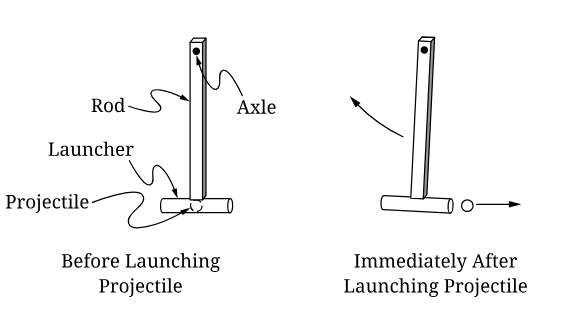
\includegraphics[width=0.8\textwidth]{6.4.1.PNG}
    \end{center}
    \item Make a Decision 
    \begin{itemize}
        \item If the p-value is less than $\alpha$, we reject the null hypothesis.
        \item If the p-value is greater than $\alpha$, we fail to reject the null hypothesis.
    \end{itemize}
    \item State the conclusion:
    \begin{itemize}
        \item Since the p-value of \blank is (less/greater) than $\alpha=\blank$, we (reject/fail to reject) the null hypothesis. There (is/is not) convincing evidence that {alternative hypothesis}.
    \end{itemize}
\end{itemize}

\begin{example}
    Jacob, an AP Statistics student, is curious to know if more male students than female students own an iPhone at his high school. He takes an SRS of 90 females and 120 male students. The survey found 
    that 61 females and 97 males owned an iPhone. Is there convincing evidence at the $\alpha=0.05$ level that more male than female students own an iPhone at Jacob's school?

    \begin{itemize}
        \item $P_M$ = true proportion of males at Jacob's HS with iPhones 
        \item $P_F$ = true proportion of females at Jacob's HS with iPhones 
    \end{itemize}

    \begin{itemize}
        \item $H_0: p_M=p_F$
        \item $H_A: p_M>p_F$
    \end{itemize}

    \begin{itemize}
        \item Random: SRS of 90 females and 120 males at Jacob's high school 
        \item Independence: $n_M=120\leq 0.10$(all males at Jacob's HS), $n_F=90\leq 0.10$(all females at Jacob's HS)
        \item Normal: $120(0.7524)=90.29\geq 10$, $120(1-0.7524)=29.71\geq 10$, $90(0.7524)=67.62\geq 10$, $90(1-0.7524)=22.28\geq 10$. Sampling dist. is approx. normal 
    \end{itemize}

    To find the $p$-value: $\hat{p}_m=\frac{97}{120}=0.8083$ and $\hat{p}_F=\frac{61}{90}=0.6778$. Plug this into the formula given above, and we get $z=2.1683$. Note that $\hat{p}_c = 0.7524$ to do this calculation.

    Using normalcdf gives us a p-value of 0.0151.

    We can also use a calculator: 

    STAT-Tests-6:2-PropZTest:
    \begin{itemize}
        \item x1: number of successes in sample of Population 1
        \item n1: sample size from Population 1
        \item x2: number of successes in sample of Population 2
        \item n2: sample size from Population 2
        \item p1: alternative hypothesis 
    \end{itemize}

    This will give the z-score and the p-value.

    Since the p-value of 0.0151 is less than $\alpha=0.05$, we reject the null. There is convincing evidence that more male than female students at Jacob's high school own an iPhone.
\end{example}


\section{Errors \& Power}
The courtroom analogy 
\begin{center}
    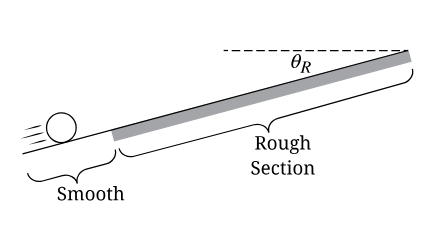
\includegraphics[width=0.8\textwidth]{6.5.1.PNG}
\end{center}

What would be considered the bigger mistake?
\begin{itemize}
    \item If the crime was murder, would a guilty person going free be the bigger mistake?
    \item If the crime was shoplifting, would and innocent person going to jail be the bigger mistake?
    \item It really comes down to the situation - statisticnas have to decide what the bigger error would be before they conduct their tests.
\end{itemize}

\begin{itemize}
    \item A jury is going to decide whether the defendant is guilty of not guilty $\rightarrow$ fail to reject or reject the null 
    \item Always start with the assumption that the defendant is innocent $\rightarrow$ assume the claim $H_0$ Is true 
    \item The court presents evidence and a decision is made $\rightarrow$ Find p-value based on a sample.
\end{itemize}

\begin{center}
    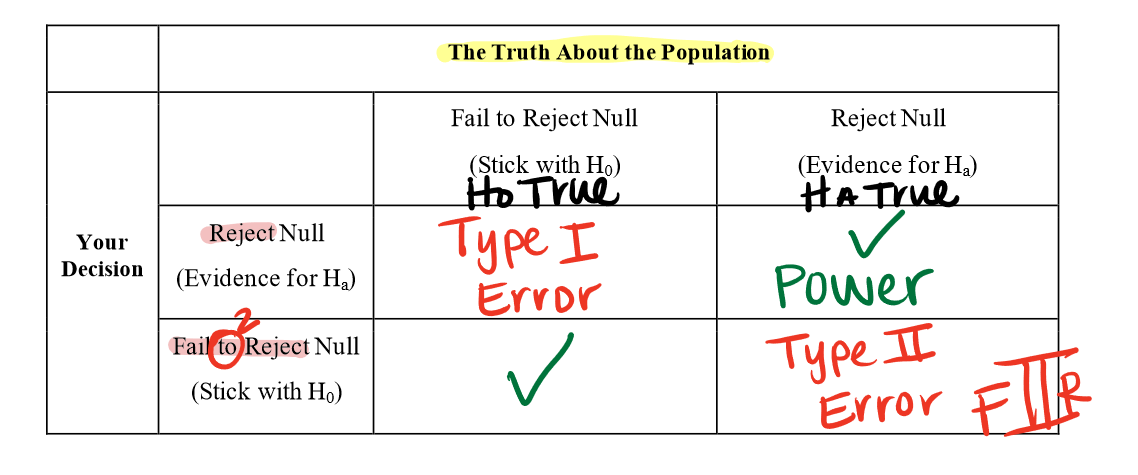
\includegraphics[width=0.8\textwidth]{6.5.2.PNG}
\end{center}

\pagebreak
\begin{example}
    $H_0:$ You are not pregnant.

    $H_A$: You are pregnant.

    When you go into a doctor's office, it is always assumed you are not pregant until we get tests that tell us otherwise.
    \begin{center}
        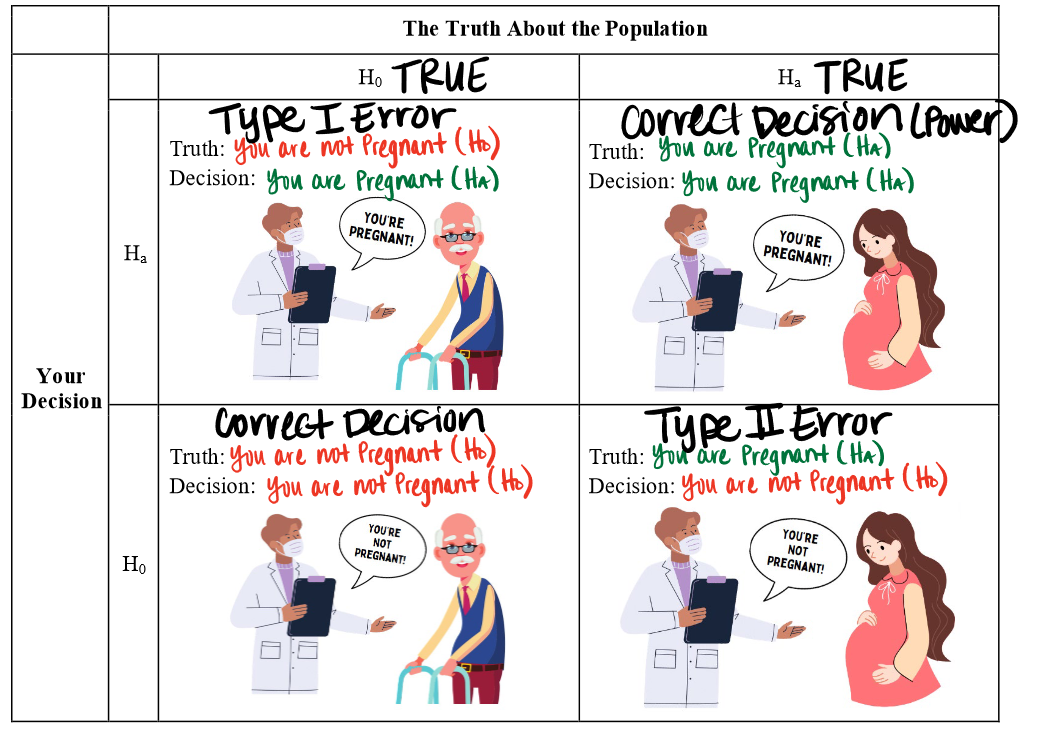
\includegraphics[width=0.8\textwidth]{6.5.3.PNG}
    \end{center}
\end{example}

Type I Error 
\begin{itemize}
    \item Reject $H_0$ incorrectly.
    \item The probability of a Type I error is equal to the significance level.
    \item P(Type I Error) = $\alpha$
    \item Our significance level tells us what p-value is ``low enough''.
\end{itemize}

Type II Error 
\begin{itemize}
    \item Fail to reject $H_0$ incorrectly 
    \item P(Type II Error) = $\beta$
\end{itemize}

Power 
\begin{itemize}
    \item Reject $H_0$ correctly 
    \item The probability we reject the null correctly is 1 minus the probability we reject the null incorrectly
    \item Power = $1-\beta$
\end{itemize}

Errors and their relationships 
\begin{itemize}
    \item Type I and Type II errors have an indirect relationship: as the probability of one increases, the probability of the other decreases.
    \item Our Type I error is set with our significance level.
    \item The higher our significancelevel is, the lower our probability of failing to reject becomes, which is why $\alpha$ and $\beta$ have an indirect relationship.
    \item The higher our significance level, the more likely we will reject the null, which increases the likelihood we do that incorrectly (as well as correctly)
    \item Therefore, Type I error and Power have a direct relationship: as the probability of Type I Error increases, the higher the Power of the test
\end{itemize}

\begin{itemize}
    \item What type of error would you rather have? Well that depends on the problem!
    \item For some tests, we want a low Type I but for others we want a low Type II.
    \item This is why being able to interpret errors is a key skill on the AP Exam.
\end{itemize}

\begin{example}
    A drug manufacturer claims that less than 10\% of patients who take its new drug for treating gestational diabetes will experience nausea. To test this claim, researchers conduct an experiment at the 5\% significance level.

    (a) What the null and alternative hypothesis?
    \begin{itemize}
        \item $H_0: p=0.10$
        \item $H_A: p<0.10$
    \end{itemize}

    (b) Describe a Type I error and a Type II error in this setting, and explain the consequences of each.

    Type I: We say less than 10\% of patients experience nausea, when really it is equal to 10\%. Manufacturer won't do anything to fix the medicine because they believe it is okay.

    Type II: We say 10\% of patients experience nausea, when really it is less than 10\%. Manufacturer will spend time to fix the drug when they don't need to.

    (c) The test has a power of 0.54 to detect that the alternative is true. Explain what the power means in this setting. What is one way we can increase the power?

    The probability we find less than 10\% of patients experiencing nausea correctly is 0.54. We can increase the power by increasing the significance level.

    (d) You know that the power of this test at the 5\% significance level against the alternative is 0.54. If you decide to usa $\alpha=0.01$ instead of the 5\% significance level, with no other changes to the test, will the power increase or decrease? Explain.

    Power will decrease because the probability we reject $H_0$ completely will decrease.
\end{example}

\end{document}